%%%%%%%%%%%%%%%%%%%%%%%%%%%%%%%%%%%%%%%%%%%%%%%%%%
\section{Liquid Argon Purity}
%%%%%%%%%%%%%%%%%%%%%%%%%%%%%%%%%%%%%%%%%%%%%%%%%%

Attenuation of the drift electron depends on purity of LAr since electronegative impurities capture it \cite{purity}. 
Thus we need to apply correction to TPC signal charge depends on the drift time.
We use cosmic ray sample triggered by inner PMT at off-beam timing for measuring the LAr purity, and use this to correct the beam data.
Figure~\ref{fig:CosmicEvent} shows an event display of typical cosmic muon event across TPC channels.
The attenuation of readout charge depending on drift time is clearly seen in the right plot. 
Readout charge in an event cannot be fitted by exponential because energy deposition follows Landau distribution and charge readout is affected by electric field distortion which is described latter in section~\ref{sec:Efield}.


%\begin{itemize}
%\item Plot: Typical Lifetime Fit  (Naganoma)
%\item Plot: Lifetime vs Time  (Naganoma)
%\end{itemize}

\begin{figure}[htbp]
 \begin{center}
  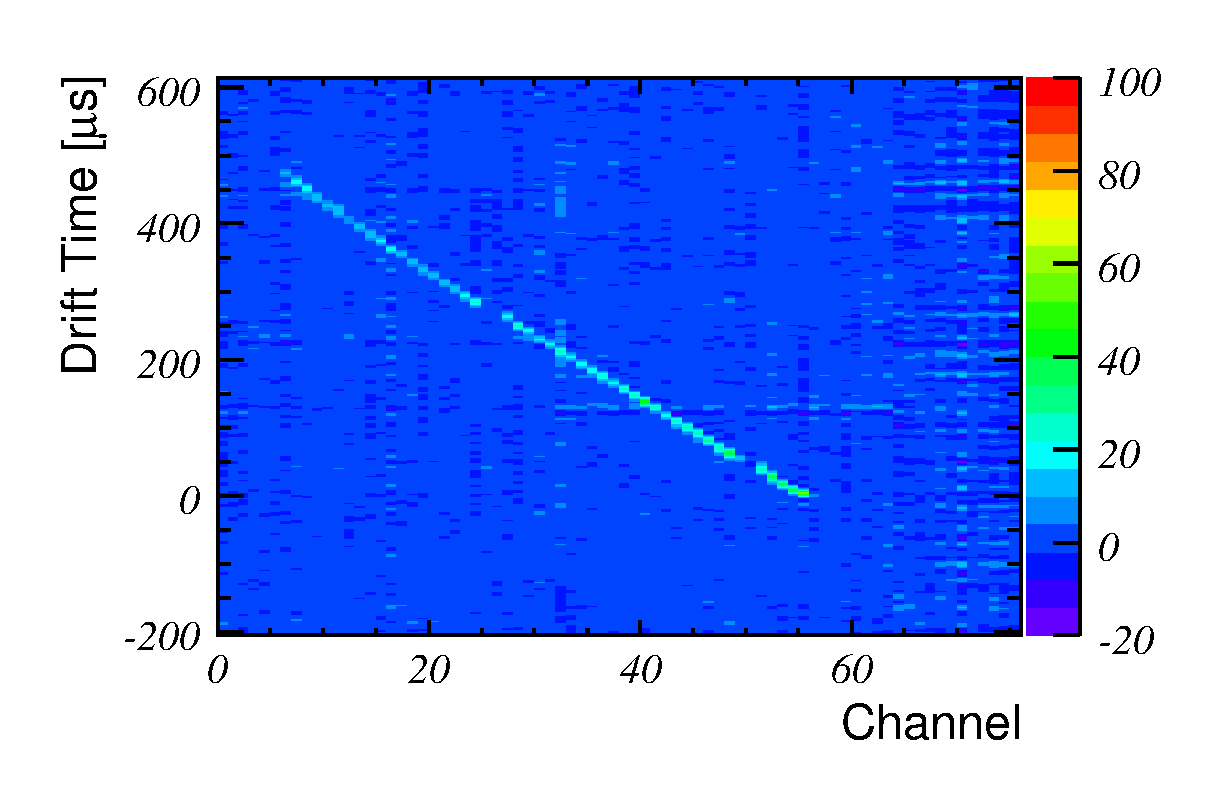
\includegraphics[width=60mm]{fig/cosmic68_ev258_display.eps}
  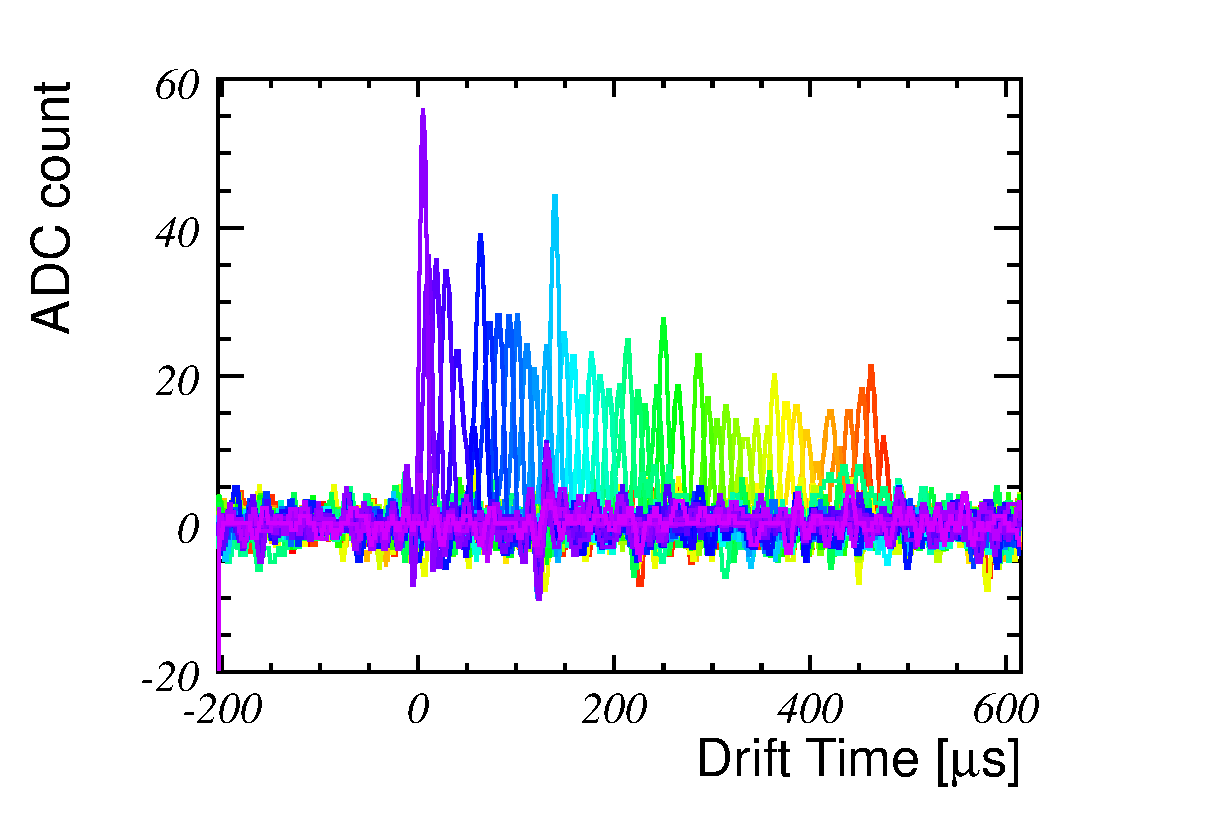
\includegraphics[width=60mm]{fig/cosmic68_ev258.eps}
 \end{center}
 \caption{Left: Typical cosmic muon event across TPC channels. Right: Charge deposit as a function of drift time. Colors correspond to different TPC channels.}
 \label{fig:CosmicEvent}
\end{figure}

We select cosmic ray event with more than 20 TPC channels which corresponds to zenith angle of more than $27^\circ$ and consistent with straight line by $\chi^2$ fit. 
Readout charge is corrected for field distortion and projected to beam direction to correct injection angle.
We fit readout charge by Landau function in each drift time bin to estimate average charge deposit. 
Figure~\ref{fig:tauExample} shows example of the average readout charge as a function of drift time is fitted by exponential to obtain drift electron lifetime. 
Realistic Monte Carlo simulation shows about 13\% (TBU) smaller lifetime estimation due to noise, field distortion, and FFT effects. 
We correct output lifetime from these effects.
Figure~\ref{fig:CosmicPurity} shows an drift electron lifetime as a function of duration after initial LAr filling.
Drift electron lifetime was 600 $\mu$s at 60 hours, and 400 $\mu$s after 150 hours.
%Initial purity looks good, but the purity was slowly degrading while data taking period.
The degradation is possibly due to impurity from micro leak or out-gassing penetrating faster than purification by gas recirculation.
But we kept enough drift electron lifetime during data taking period.

\begin{figure}[htbp]
 \begin{center}
  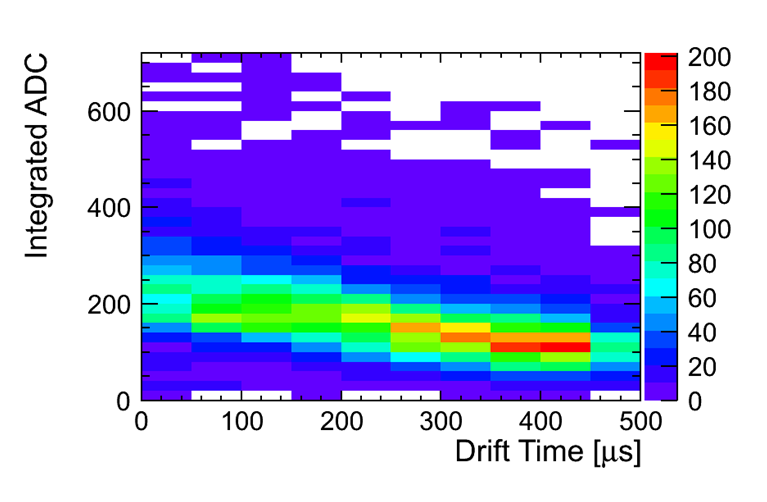
\includegraphics[width=60mm]{fig/chargeDep.eps}
  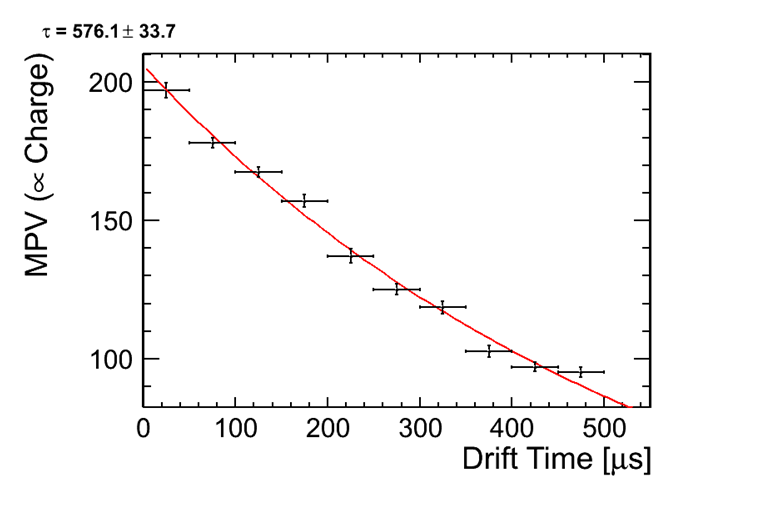
\includegraphics[width=60mm]{fig/tauExample.eps}
 \end{center}
 \caption{TBU. Left: Readout charge as a function of drift time. Readout charge in each drift time bin is fitted by landau function. Right: Average charge readout as a function of drift time which is fitted by exponential to estimate drift electron lifetime.}
 \label{fig:tauExample}
\end{figure}


\begin{figure}[htbp]
 \begin{center}
  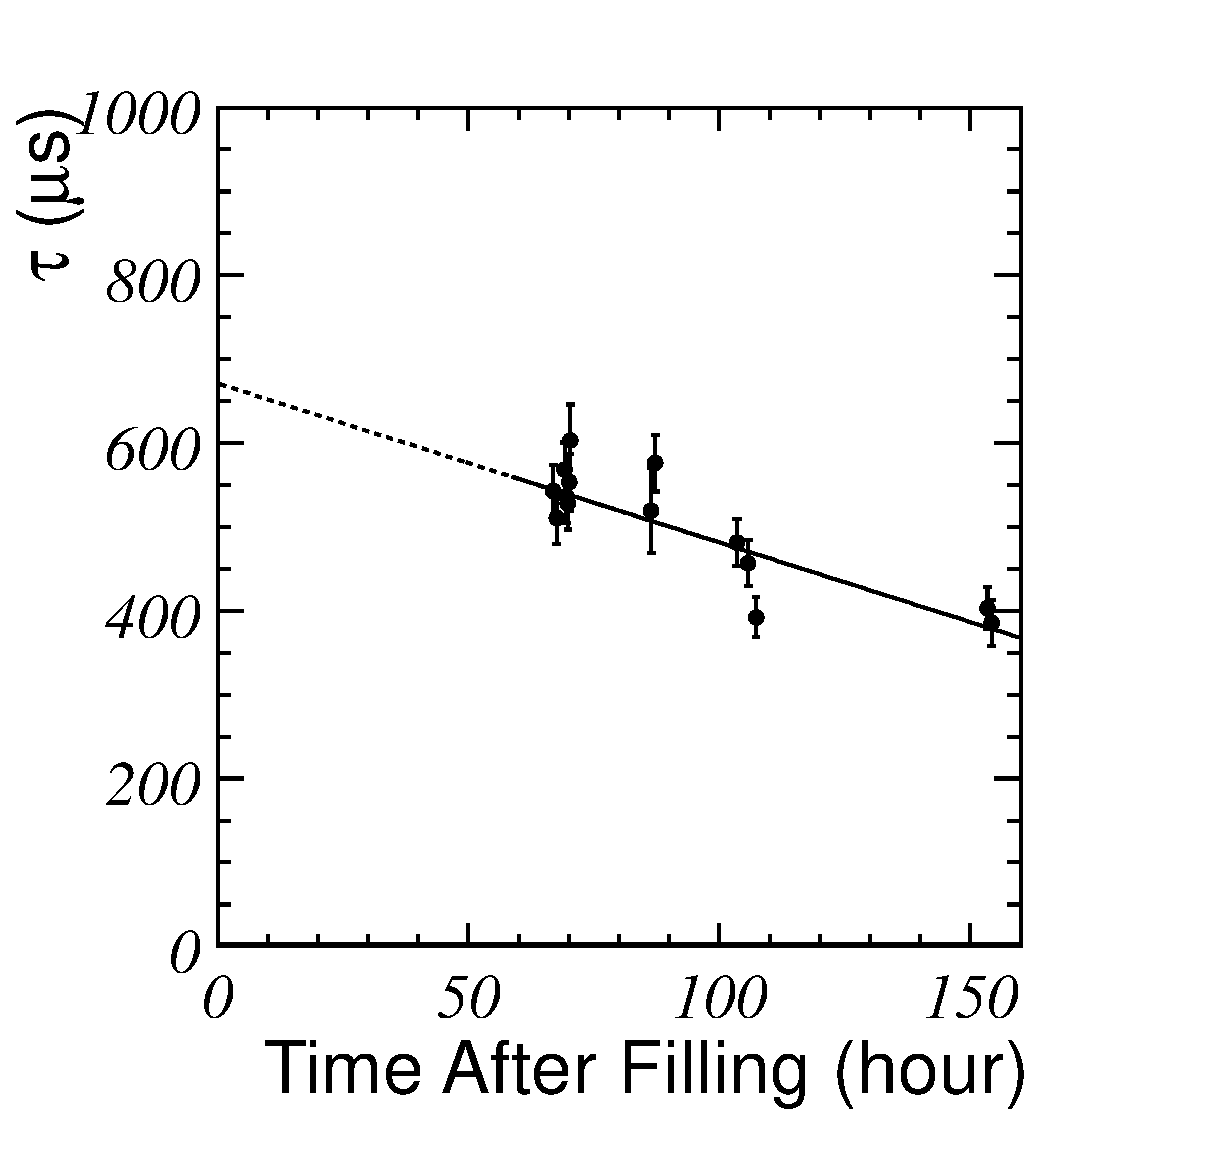
\includegraphics[width=60mm]{fig/tauHistory.eps}
 \end{center}
 \caption{TBU. Drift electron lifetime as a function of duration after initial LAr filling. The lifetime is used to correct the beam data.}
 \label{fig:CosmicPurity}
\end{figure}

